\section{Tool-chain capabilities}
The tool-chain support matrix depicts available platform support on current open-source projects. Projects that rely on these tool-chains like APIO or icestudio are not represented as their features are already covered.
Based on the current project progress, implemented features are shown in tables \ref{basic-tiles}, \ref{advanced-tiles} and \ref{routing}

\begin{table}[htp]
\centering
\begin{tabular}{|l|c|c|c|}
\hline
       & \multicolumn{1}{l|}{\textbf{IceStorm}} & \multicolumn{1}{l|}{\textbf{Trellis}} & \multicolumn{1}{l|}{\textbf{X-Ray}} \\ \hline
\textbf{Logic}     & Yes     & Yes & Yes \\ \hline
\textbf{Block RAM} & Yes & Yes & Partial \\ \hline
\end{tabular}
\caption{Basic Tiles}
\label{basic-tiles}
\end{table}


\begin{table}[htp]
\centering
\begin{tabular}{|l|c|c|c|}
\hline
                     & \multicolumn{1}{l|}{\textbf{IceStorm}} & \multicolumn{1}{l|}{\textbf{Trellis}} & \multicolumn{1}{l|}{\textbf{X-Ray}} \\ \hline
\textbf{DSP}         & Yes                                    & Yes                                   & No                                  \\ \hline
\textbf{Hard Blocks} & Yes                                    & Yes                                   & No                                  \\ \hline
\textbf{Clock Tiles} & Yes                                    & Yes                                   & No                                  \\ \hline
\textbf{I/O Tiles}   & Yes                                    & Yes                                   & Partial                             \\ \hline
\end{tabular}
\caption{Advanced Tiles}
\label{advanced-tiles}
\end{table}


\begin{table}[htp]
\centering
\begin{tabular}{|l|c|c|c|}
\hline
       & \multicolumn{1}{l|}{\textbf{IceStorm}} & \multicolumn{1}{l|}{\textbf{Trellis}} & \multicolumn{1}{l|}{\textbf{X-Ray}} \\ \hline
\textbf{Logic}     & Yes     & Yes & Yes \\ \hline
\textbf{Clock} & Yes & Yes & No \\ \hline
\end{tabular}
\caption{Routing}
\label{routing}
\end{table}

Tool-chain features for open-source and free software is shown in Table \ref{features}

\begin{table}
\begin{tabular}{|l|l|l|l|l|l|l|}
\hline
\textbf{}           & \textbf{IDE} & \textbf{\begin{tabular}[c]{@{}l@{}}Block \\ Design\end{tabular}} & \textbf{\begin{tabular}[c]{@{}l@{}}Timing\\ Analysis\end{tabular}} & \textbf{Simulation} & \textbf{\begin{tabular}[c]{@{}l@{}}Pin Mapping \\ GUI\end{tabular}} & \textbf{\begin{tabular}[c]{@{}l@{}}Floorplan \\ GUI\end{tabular}} \\ \hline
\textbf{APIO}       & Yes          & No                                                               & Yes                                                                & Yes                 & No                                                                  & No                                                                \\ \hline
\textbf{icestorm}   & No           & No                                                               & External                                                           & External            &                                                                     &                                                                   \\ \hline
\textbf{icestudio}  & Yes          & Yes                                                              & No                                                                 & No                  & No                                                                  & No                                                                \\ \hline
\textbf{prjtrellis} & No           & No                                                               &                                                                    &                     &                                                                     &                                                                   \\ \hline
\textbf{Quartus}    & Yes          & Yes                                                              & Yes                                                                & Yes                 & Yes                                                                 & Yes                                                               \\ \hline
\textbf{Vivado}     & Yes          & Yes                                                              & Yes                                                                & Yes                 & Yes                                                                 & Yes                                                               \\ \hline
\end{tabular}
\caption{Features}
\label{features}
\end{table}

\section{icestorm and prjtrellis}

These are command line tools for ICE40 and ECP5 FPGA series. Each tool is responsible for a single step in the process of taking a verilog file and ending up with a programmed device. Since this is a multistep process, it is best to be carried out by using a Makefile as demonstrated in the project repository.

There is a PLL configuration tool for each platform (icepll, ecppll) that can be used for generating PLL code. As en example an 120MHz clock derived from a 12MHz clock is demonstrated:

\begin{tcolorbox}
\begin{verbatim}
$ icepll -m -f pll.v -i 12 -o 120

F_PLLIN:    12.000 MHz (given)
F_PLLOUT:  120.000 MHz (requested)
F_PLLOUT:  120.000 MHz (achieved)

FEEDBACK: SIMPLE
F_PFD:   12.000 MHz
F_VCO:  960.000 MHz

DIVR:  0 (4'b0000)
DIVF: 79 (7'b1001111)
DIVQ:  3 (3'b011)

FILTER_RANGE: 1 (3'b001)

PLL configuration written to: pll.v

\end{verbatim}
\end{tcolorbox}
This will also generate a pll module file that can be included in the project

\begin{tcolorbox}
\begin{verbatim}
/**
 * PLL configuration
 *
 * This Verilog module was generated automatically
 * using the icepll tool from the IceStorm project.
 * Use at your own risk.
 *
 * Given input frequency:        12.000 MHz
 * Requested output frequency:  120.000 MHz
 * Achieved output frequency:   120.000 MHz
 */

module pll(
	input  clock_in,
	output clock_out,
	output locked
	);

SB_PLL40_CORE #(
		.FEEDBACK_PATH("SIMPLE"),
		.DIVR(4'b0000),		// DIVR =  0
		.DIVF(7'b1001111),	// DIVF = 79
		.DIVQ(3'b011),		// DIVQ =  3
		.FILTER_RANGE(3'b001)	// FILTER_RANGE = 1
	) uut (
		.LOCK(locked),
		.RESETB(1'b1),
		.BYPASS(1'b0),
		.REFERENCECLK(clock_in),
		.PLLOUTCORE(clock_out)
		);

endmodule

\end{verbatim}
\end{tcolorbox}

Timing analysis is available for ICE40 using the icetime tool. It will report timing estimate as well as detailed timing report.

Simulation is possible by creating a testbench file and using iverilog combined with gtk-wave for visualization



\section{APIO}
APIO is a command line tool that wraps around icestorm toolchain and attempts to simplify development process. It provides all features of icestorm toolchain as well as simulation. It handles driver installation and project initialization for supported boards.

A summary of available features is presented by command usage
\begin{tcolorbox}
\begin{verbatim}
Project commands:
  build      Synthesize the bitstream.
  clean      Clean the previous generated files.
  lint       Lint the verilog code.
  sim        Launch the verilog simulation.
  time       Bitstream timing analysis.
  upload     Upload the bitstream to the FPGA.
  verify     Verify the verilog code.

Setup commands:
  drivers    Manage FPGA boards drivers.
  init       Manage apio projects.
  install    Install packages.
  uninstall  Uninstall packages.

Utility commands:
  boards     Manage FPGA boards.
  config     Apio configuration.
  examples   Manage verilog examples.
  raw        Execute commands using Apio packages.
  system     System tools.
  upgrade    Check the latest Apio version.
\end{verbatim}
\end{tcolorbox}
One drawback is that it uses the now deprecated arachne-pnr instead of its replacement nextpnr.

An Atom editor plugin is available that integrates APIO functionality and provides the same functionality from within the editor.
\begin{figure}[h!]
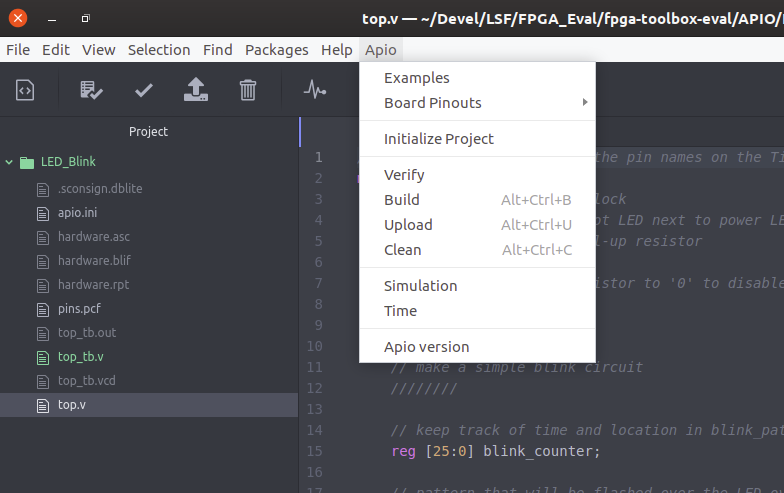
\includegraphics[width=1\textwidth]{Images/APIO_Atom.png}
\caption{APIO plugin for Atom}
\end{figure}
\section{IceStudio}
Icestudio is built on top of APIO and Icestorm projects and currently supports the ICE40 FPGA family. Icestudio comes as an AppImage and handles all toolchain and "Driver" (udev rules) requirements through its GUI
It is a block design editor (Figure \ref{ref:icestudio_block}) and comes with a basic set of blocks like

\begin{itemize}
\item I/O
\item Memory
\item Multiplexers
\item Gates
\item Flip-flops
\item Prescalers/Counters
\end{itemize}

\begin{figure}[ht]
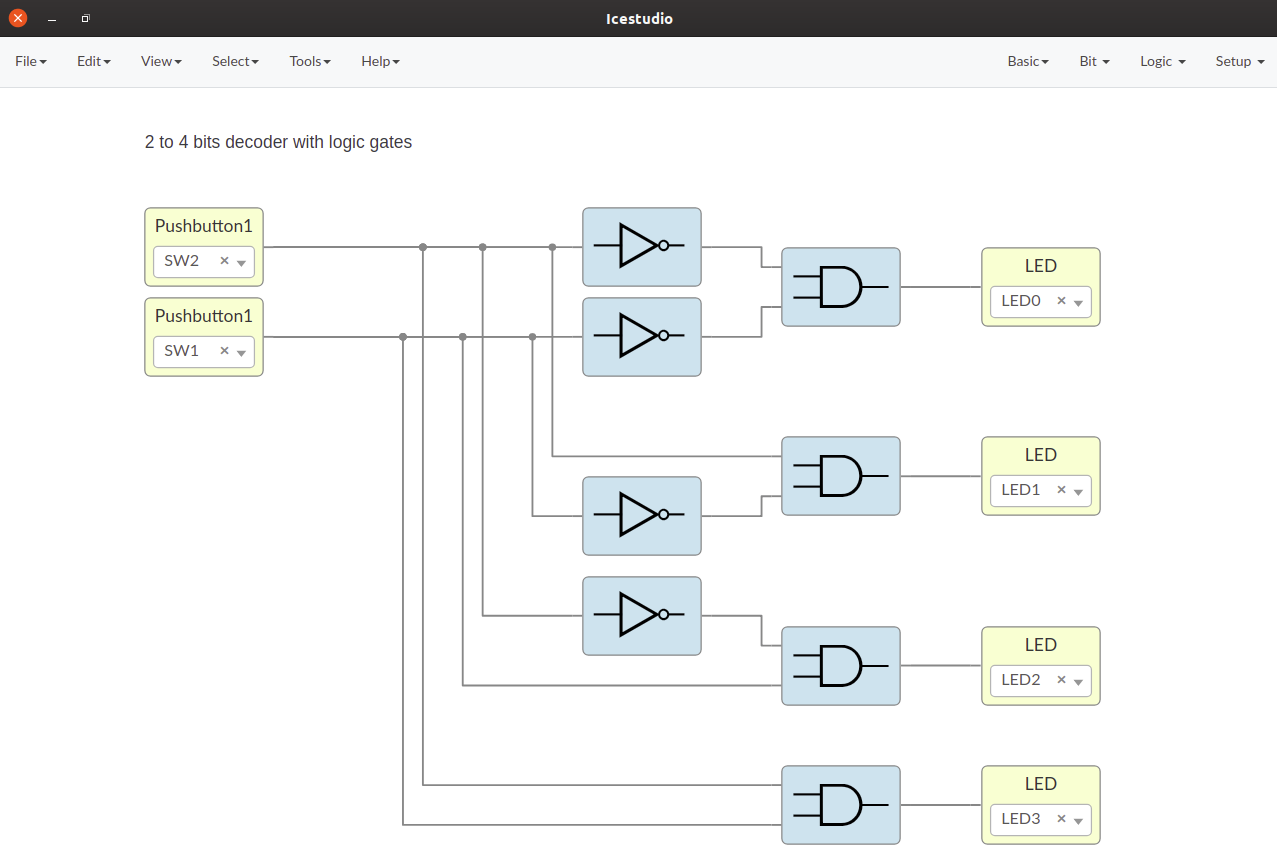
\includegraphics[width=1\textwidth]{Images/icestudio_blocks.png}
\caption{Icestudio block design}
\label{ref:icestudio_block}
\end{figure}

Custom blocks can be created by implementing the underlying functionality in Verilog (Figure \ref{ref:icestudio_custom_block}) and provide input and output ports in order to connecto to other blocks
\begin{figure}[ht]
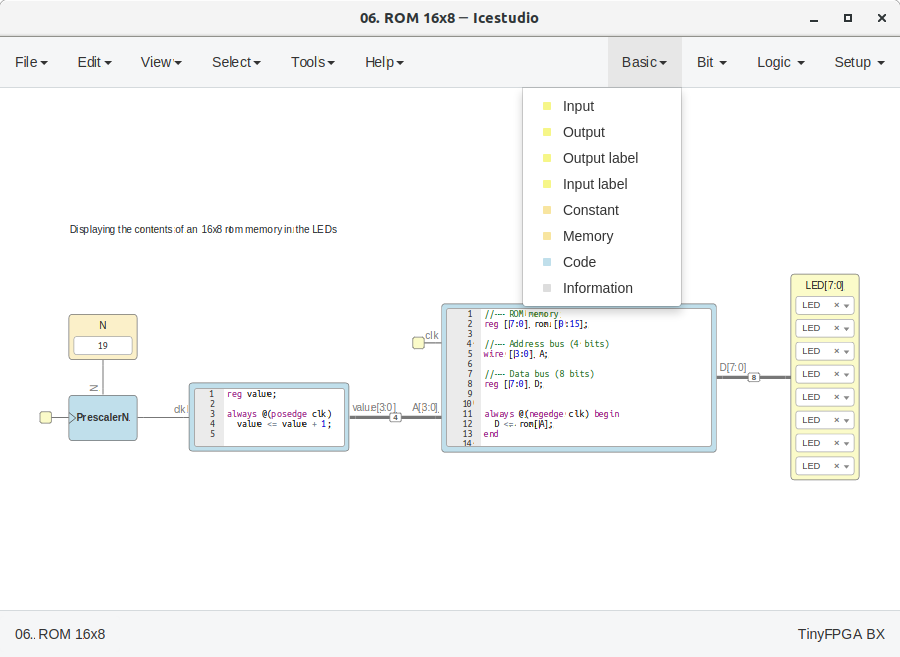
\includegraphics[width=1\textwidth]{Images/icestudio_custom_block.png}
\caption{Icestudio custom block}
\label{ref:icestudio_custom_block}
\end{figure}

Sets of blocks can be organised in collections that are ZIP files of specific file structure. Collections can be added in Icestudio extending its functionality. Collections also include example projects that can be loaded into the block editor

A list of opensource collections can be found at 

\url{https://github.com/FPGAwars/icestudio-collections}

\url{https://fpgawars.github.io/}

For creating custom collections, a tool is available assisting in creating the basic file and folder structure: \url{https://github.com/FPGAwars/icm}

\section{Quartus}
Quartus supports VHDL and Verilog source files as well as block design. It comes with a variety of IP core re-configurable generators

Quartus Prime software features include \cite{Wikipedia_Quartus}:
\begin{itemize}
\item SOPC Builder, a tool in Quartus Prime software that eliminates manual system integration tasks by automatically generating interconnect logic and creating a testbench to verify functionality
\item Qsys, a system-integration tool that is the next generation of SOPC Builder. It uses an FPGA-optimized network-on-chip architecture that doubles the fMAX performance vs. SOPC Builder.
\item SoCEDS, a set of development tools, utility programs, run-time software, and application examples to help you develop software for SoC FPGA embedded systems.
\item DSP Builder, a tool that creates a seamless bridge between the MATLAB/Simulink tool and Quartus Prime software, so FPGA designers have the algorithm development, simulation, and verification capabilities of MATLAB/Simulink system-level design tools
\item External memory interface toolkit, which identifies calibration issues and measures the margins for each DQS signal.
\item Generation of JAM/STAPL files for JTAG in-circuit device programmers.
\end{itemize}

A comparison of available features at this time is shown in 

\section{Vivado}
Vivado HL WebPACK Edition was used for this evaluation. It is provided at no cost but with device limitations.

Features available in this edition are:
\begin{itemize}
    \item Synthesis and Place and Route
    \item Dynamic Function eXchange
    \item Simulator
    \item Device Programmer
    \item Logic Analyzer
    \item Serial I/O Analyzer
    \item Debug IP (ILA/VIO/IBERT)	\item High-Level Synthesis
    \item IP Integrator
\end{itemize}

Non free editions also include System Generator for DSP and Model Composer